\documentclass[10pt]{beamer}

\usetheme{metropolis}
\usepackage{appendixnumberbeamer}

\usepackage{verbatim}
\usepackage{subfigure}
\usepackage{caption}
\usepackage{graphicx}
\usepackage{epstopdf}

\usepackage{booktabs}
\usepackage[scale=2]{ccicons}

\usepackage{pgfplots}
\usepgfplotslibrary{dateplot}

\usepackage{xspace}
\newcommand{\themename}{\textbf{\textsc{metropolis}}\xspace}

\title{FEP Index Matching}
\subtitle{Index Matching}
\date{\today}
\author{Greg Sakradse}

\begin{document}


\begin{frame}{Blur Factor Plots: NaCl}
\begin{figure}
    \centering
    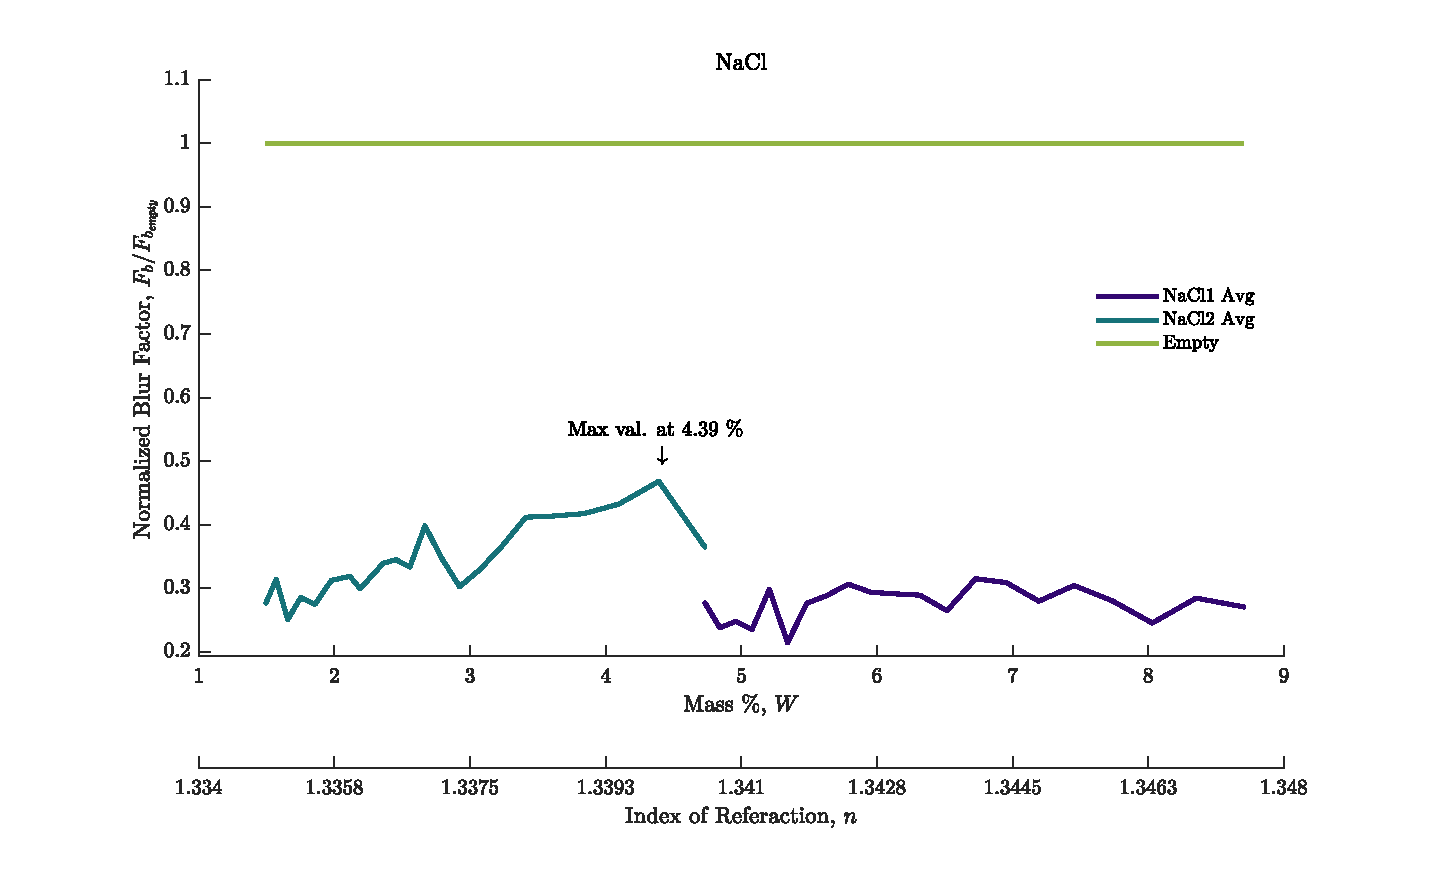
\includegraphics[width = 0.75 \textwidth]{figs/NaCl_BlurPlot.eps}
    \label{NaClBlur}
\end{figure}
    
\end{frame}

\begin{frame}{Blur Factor Plots: Glycerol}
\begin{figure}
    \centering
    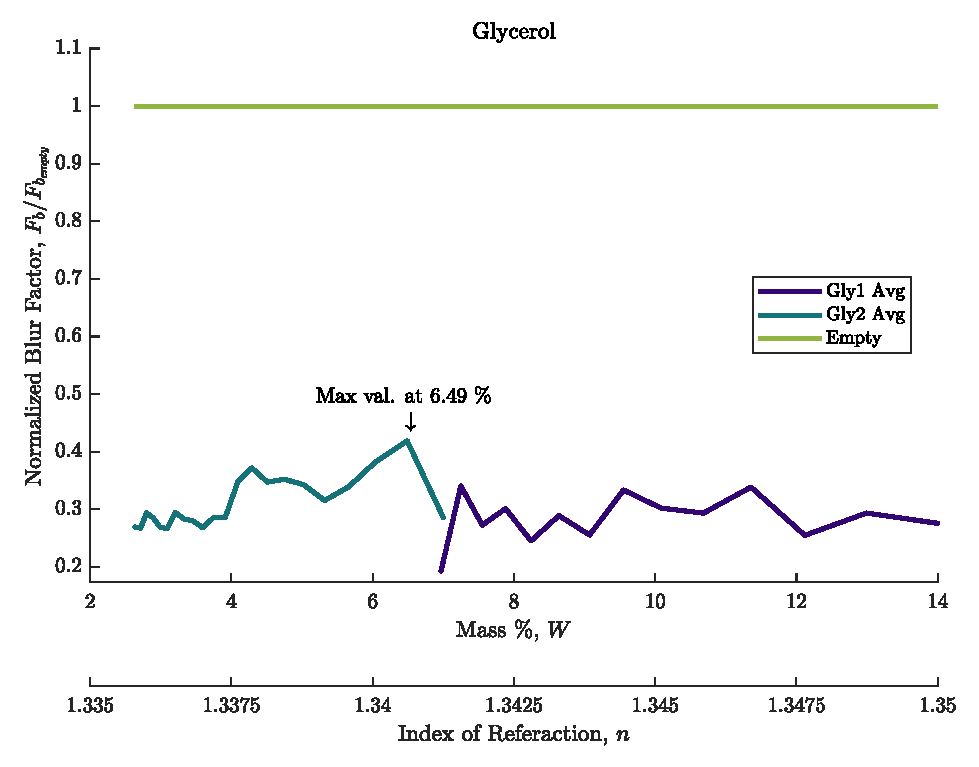
\includegraphics[width = 0.75\textwidth]{figs/Gly_BlurPlot.eps}
    \label{GlyBlur}
\end{figure}
    
\end{frame}

\begin{frame}{NaCl Images}
\begin{figure}
    \centering
<<<<<<< HEAD
    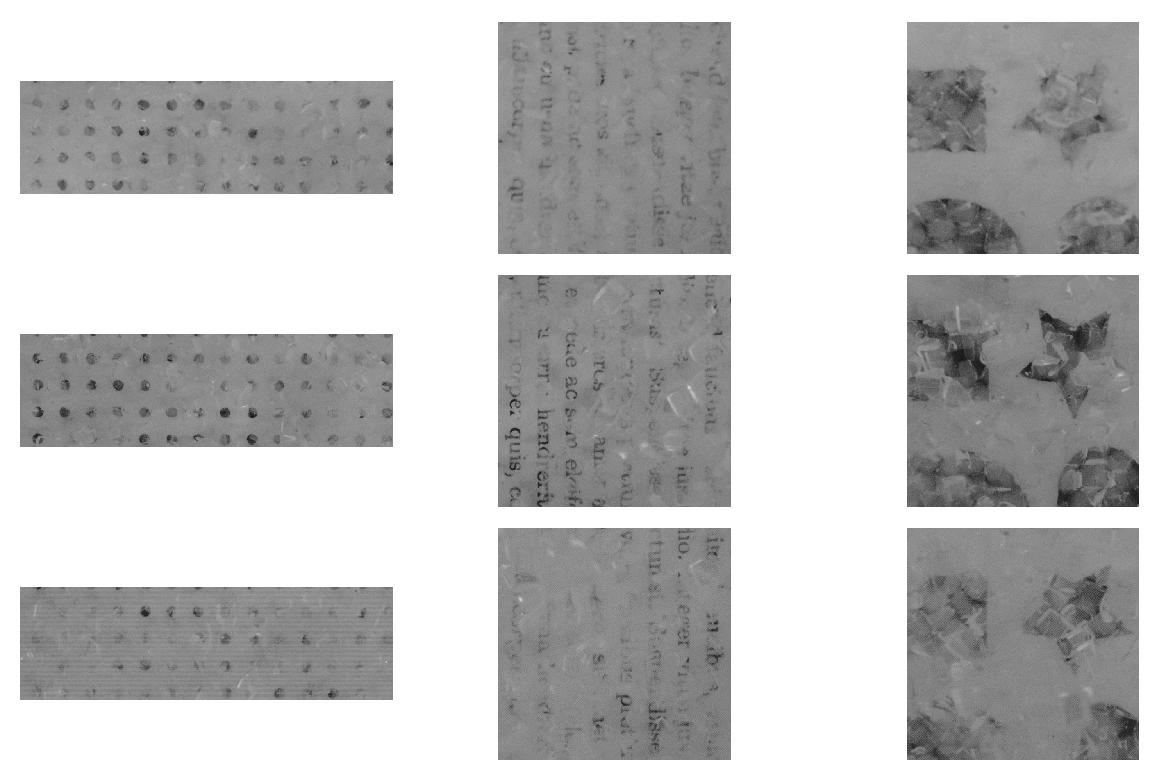
\includegraphics[width = 0.75\textwidth]{figs/NaCl_Imgs002.eps}
=======
    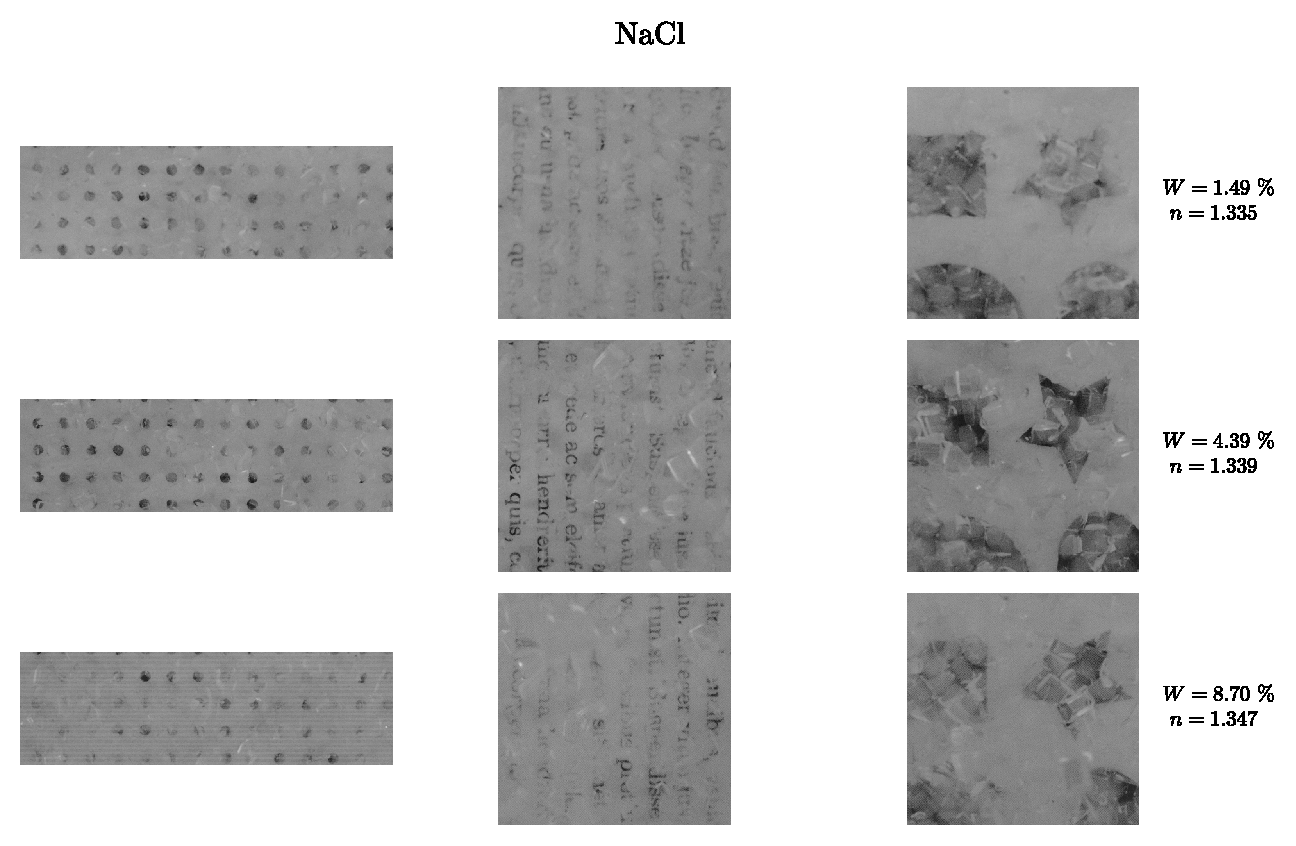
\includegraphics[width = 0.75\textwidth]{figs/NaCl_Imgs.eps}
>>>>>>> master
    \label{NaClImg}
\end{figure}
\end{frame}

\begin{frame}{Glycerol Images}
\begin{figure}
    \centering
<<<<<<< HEAD
    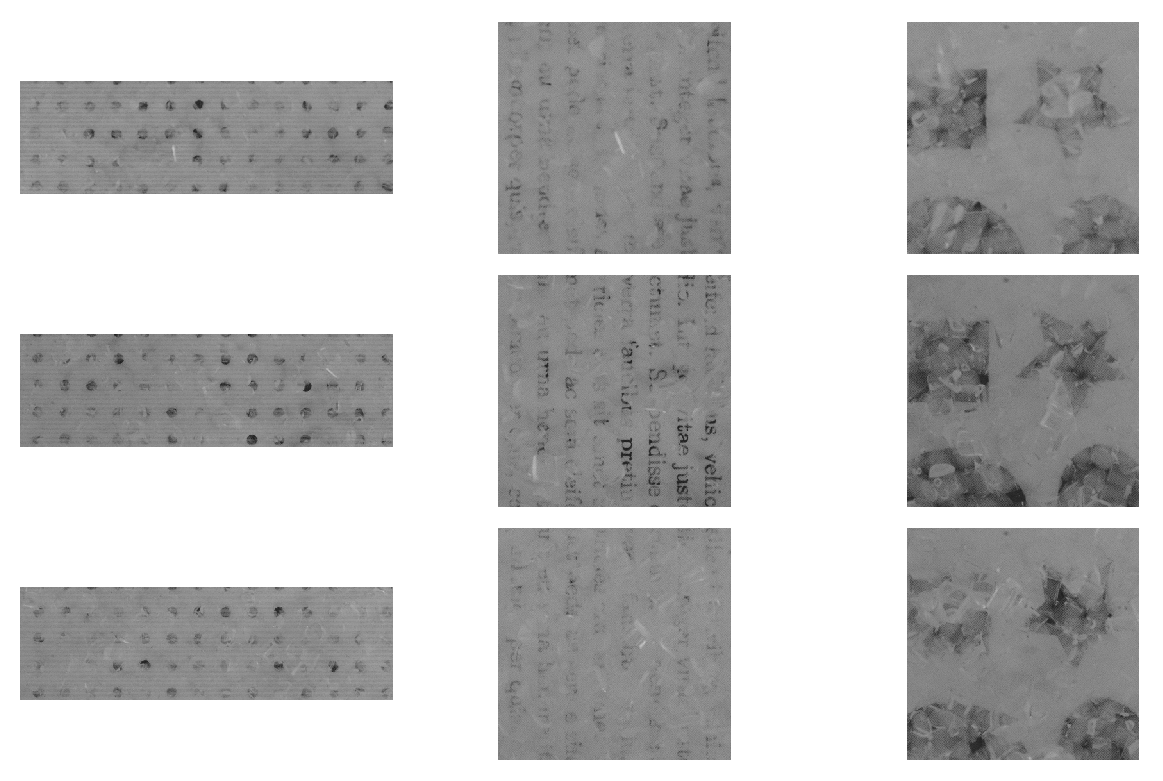
\includegraphics[width = 0.75\textwidth]{figs/Gly_Imgs002.eps}
    \label{Glyshapes}
=======
    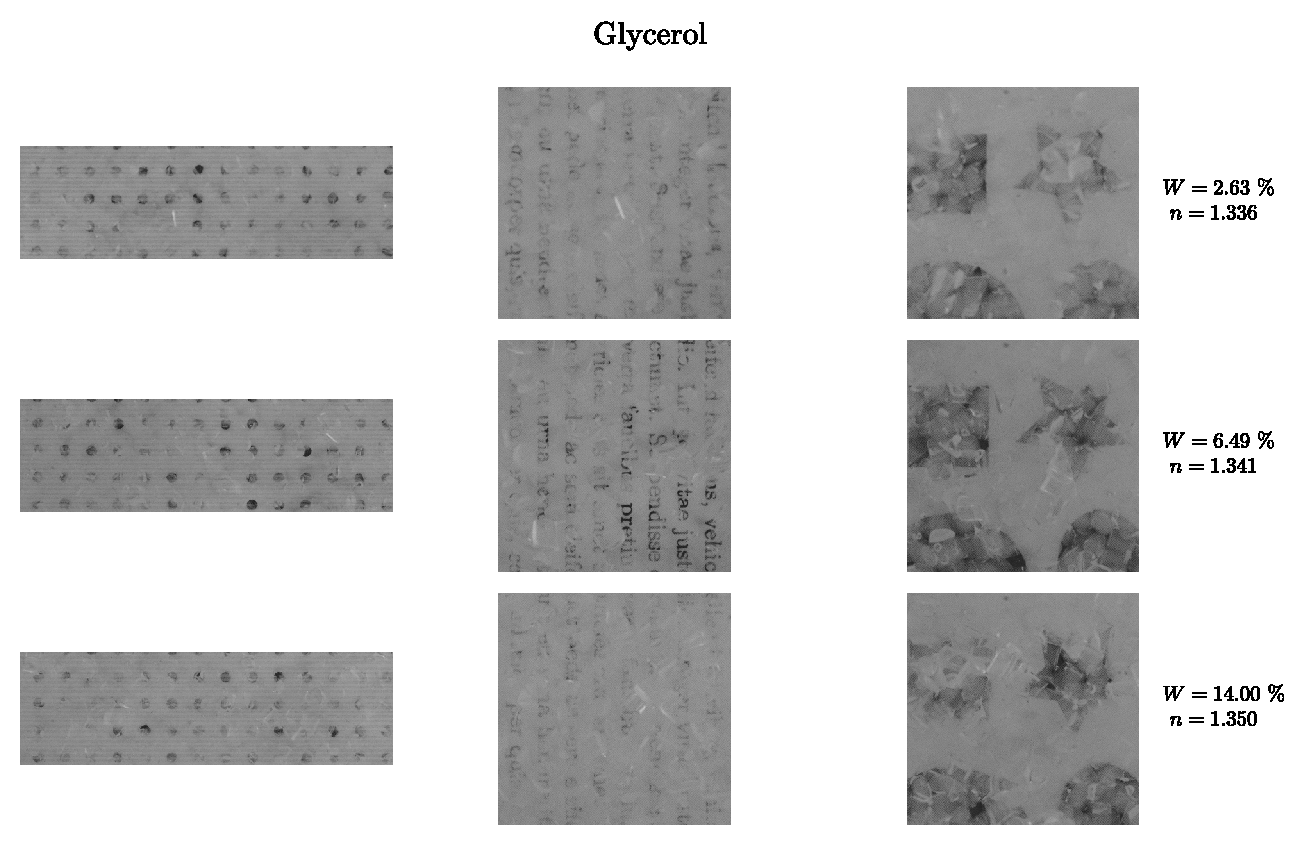
\includegraphics[width = 0.75\textwidth]{figs/Gly_Imgs.eps}
    \label{ex_shapes}
>>>>>>> master
\end{figure}
    
\end{frame}


\end{document}
